\chapter{Design and Modeling of the Digital Twin}
\label{chap:chapter3}

This chapter presents the five-layer architecture of the digital twin system, describes the 3D model developed in Blender, explains the behavioural model that integrates physics-based rules with machine learning techniques, and details how all components remain synchronised in real time.

\section{Overall System Architecture}

The system follows a five-layer architecture (Table~\ref{tab:five_layer_architecture}) adapted from Tao et al.~\cite{Tao2019} for edge-first deployment on a BCN3D+ FDM printer. Each layer corresponds to a distinct functional responsibility, from physical signal generation to operator-facing dashboards.

\begin{table}[H]
\centering
\caption{Five-layer architecture summary}
\begin{tabular}{|L{2.8cm}|L{3.0cm}|L{4.0cm}|L{4.5cm}|}
	\hline
	\rowcolor{primary}
	\textbf{\color{white}Layer} & \textbf{\color{white}Name} & \textbf{\color{white}Components / Technologies} & \textbf{\color{white}Primary Function} \\
	\hline
	1 & Physical & BCN3D+ printer, KY-013 thermistor, MPU-6050 IMU, OctoPrint end-stops , filament mouse encoder & Generate raw sensor and firmware signals \\
	\hline
	2 & IoT / Acquisition & ESP8266 sensor node, Raspberry Pi gateway, Mosquitto broker & Acquire, condition, and transmit sensor data \\
	\hline
	3 & Data Processing & data\_aligner.py, feature\_engineering.py, PMx AI pipeline & Align, clean, feature-engineer, and classify fault signals \\
	\hline
	4 & Virtual Model & Blender 3D geometric model, Three.js renderer, ML engine & Maintain live 3D replica + health state of physical printer \\
	\hline
	5 & Supervision & React/Vite dashboard, alert engine, print session history & Present real-time DT state, alerts, and decisions to operator \\
	\hline
\end{tabular}
\label{tab:five_layer_architecture}
\end{table}

\subsection{C4 Model Decomposition}

Figure~\ref{fig:c4_context} shows the system context. Two external actors interact with the digital twin: the \textbf{Operator} (monitors the dashboard, acknowledges alerts) and the \textbf{Technician} (performs physical maintenance guided by predictive recommendations). The physical printer (BCN3D+) streams telemetry via MQTT~\cite{mqtt5_spec} and receives control commands (e.g., print pauses) when faults are detected.

\begin{figure}[H]
    \centering
    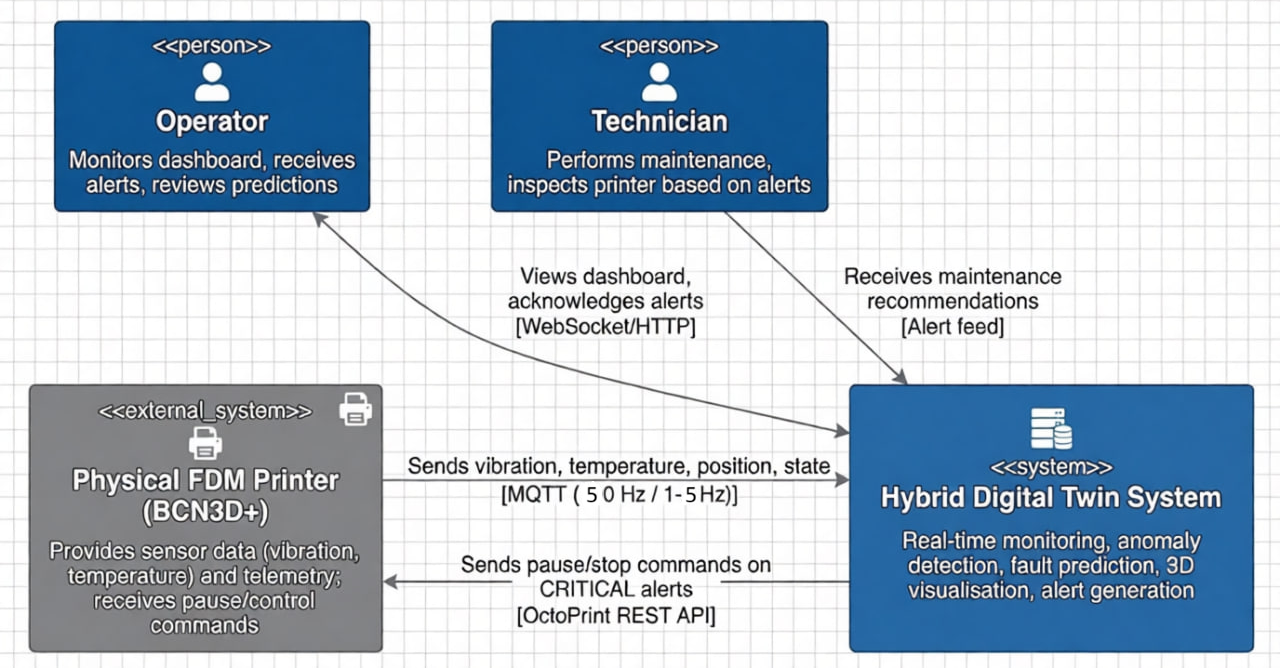
\includegraphics[width=0.9\textwidth]{figures/diagram_c4_context}
    \caption{C4 Context Diagram: external actors and the digital twin system}
    \label{fig:c4_context}
\end{figure}

Internally, the C4 Container diagram (Figure~\ref{fig:c4_container}) identifies five software containers. The \texttt{ESP8266 Sensor Node}~\cite{esp8266_trm} and \texttt{OctoPrint} publish raw sensor streams (IMU, thermistor, filament encoder) to an \texttt{Mosquitto MQTT broker}. A \texttt{Python Backend} subscribes, aligns timestamps, engineers features, and runs the fault detection ensemble. Processed states and alerts are pushed via WebSocket to a \texttt{React + Three.js dashboard}, which renders a live 3D printer replica. Prior work validates that Three.js combined with MQTT and WebSocket achieves sub-second update latencies (280--550~ms) suitable for real-time monitoring~\cite{pmc2025building}. Persistent storage of telemetry and engineered features is handled by local SQLite databases~\cite{sqlite2024}.

\begin{figure}[H]
    \centering
    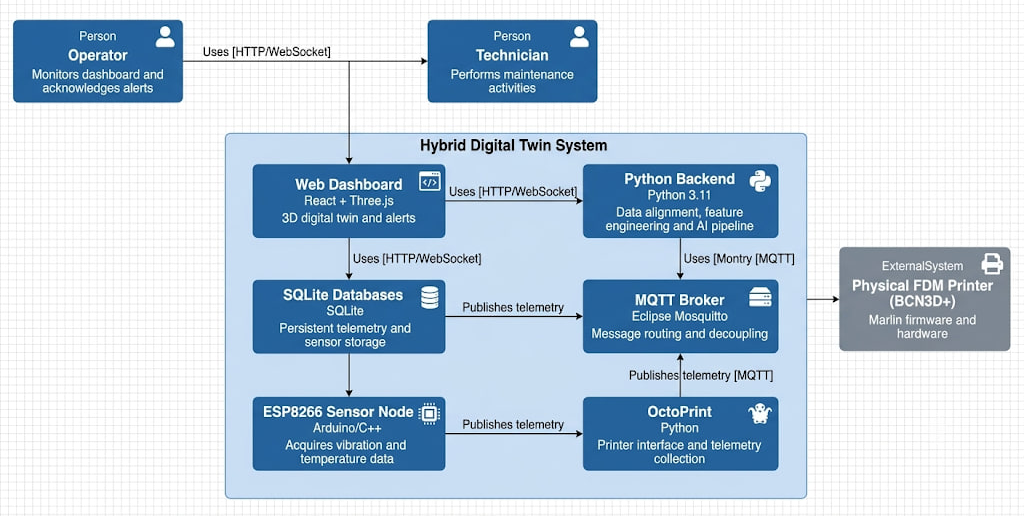
\includegraphics[width=0.9\textwidth]{figures/diagram_c4_container}
    \caption{C4 Container Diagram: main software containers}
    \label{fig:c4_container}
\end{figure}

\subsection{Five-Dimensional Digital Twin Mapping}

Figure~\ref{fig:dt_5d} maps the architecture onto the five-dimensional digital twin model proposed by Tao et al.~\cite{Tao2019}. The \textbf{Physical Entity (PE)} is the BCN3D+ printer with three attached sensors (IMU, thermistor, optical encoder). The \textbf{Virtual Entity (VE)} consists of (1) a geometric 3D model (Three.js) and (2) a behavioural model comprising three binary classifiers (extrusion, vibration, thermal) and a Health Index. \textbf{Connections (CN)} are bidirectional: MQTT for telemetry uplink, WebSocket for state downlink. \textbf{Twin Data (DD)} stores raw and engineered features in local SQLite databases. \textbf{Services (Ss)} expose monitoring (dashboard), prediction (fault probabilities), and control (print pause) functions.

\begin{figure}[H]
    \centering
    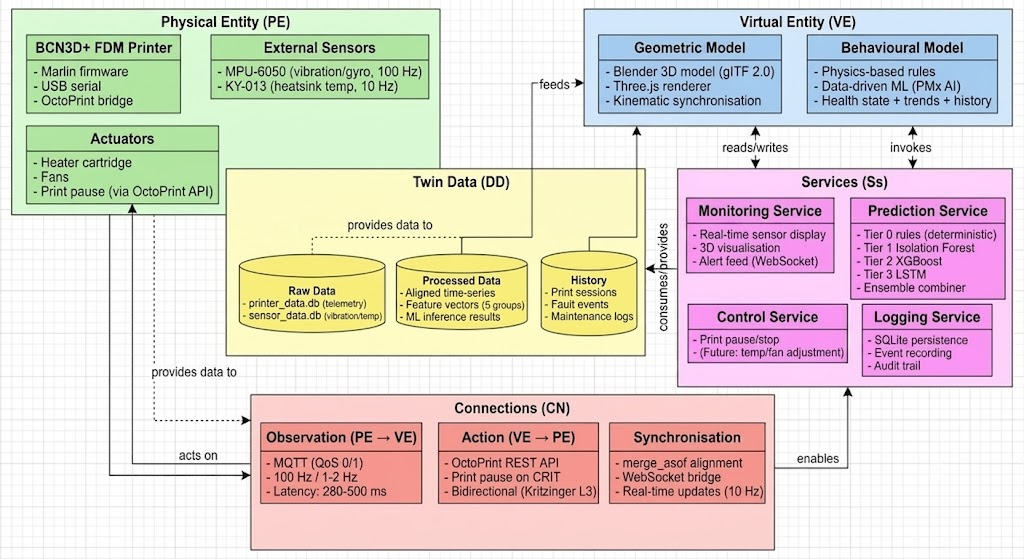
\includegraphics[width=0.9\textwidth]{figures/diagram_dt_5d}
    \caption{Five-dimensional digital twin model (Tao et al.) applied to this work}
    \label{fig:dt_5d}
\end{figure}

\subsection{Layer 1: Physical Layer}

The physical asset is a BCN3D+ printer with dual extruders, a RAMPS 1.4 board, and Marlin 1.x firmware. External sensors include a KY-013 thermistor on the heatsink (sampling at 2 Hz) and an MPU-6050 IMU on the X-carriage (sampling at 50 Hz), filament encoder between the spool and extruding model. Built-in sensors (like the nozzle thermistor and end-stops) are accessed through OctoPrint \cite{octoprint2024api}. Actuators (heater, fans, print pause) are controlled via OctoPrint's REST API, which enables bidirectional digital twin capability.

\subsection{Layer 2: Acquisition / IoT Layer}

An ESP8266 microcontroller samples the sensors, computes changes (deltas), and publishes JSON data via MQTT (using QoS 0 for regular telemetry and QoS 1 for alerts). A Mosquitto broker runs on a Raspberry Pi. Python collectors then store the data in two SQLite databases.

\subsection{Layer 3: Data Processing Layer}

This layer handles cleaning the data, aligning timestamps, engineering features, and running the three-tier PMx AI pipeline.

\subsubsection{Data Alignment}
The \verb|data_aligner.py| script loads both databases, shifts sensor timestamps backward by 200 milliseconds to compensate for MQTT latency, and uses Pandas \texttt{merge\_asof} function with a tolerance window of ±500 milliseconds \cite{mckinney2010data}.

\subsubsection{Feature Engineering}
The \verb|feature_engineering.py| script extracts five groups of features:

\begin{itemize}
    \item \textbf{Group A (thermal):} nozzle error, heatsink slope (rate of temperature change over time)
    \item \textbf{Group B (vibration):} RMS, kurtosis, crest factor from the MPU-6050 sensor
    \item \textbf{Group C (spectral):} dominant frequency and band power (reserved for future use)
    \item \textbf{Group D (context):} extrusion state, feedrate
    \item \textbf{Group E (cross-source):} vibration per feedrate, nozzle error during extrusion
\end{itemize}

Table~\ref{tab:feature_engineering} details the five feature groups. For each group, the table lists the source sensor, the extracted features, and the fault mode targeted by those features. For example, Group A targets overheating and heat creep using thermal features from the KY-013 sensor, while Group B targets nozzle clogging and bearing wear using vibration features from the MPU-6050.

\begin{table}[H]
\centering
\caption{Feature engineering groups}
% ============================================================
% TABLE: Feature Engineering Groups
% ============================================================
{
\scriptsize
\rowcolors{2}{white}{primary!10}

\begin{tabular}{|L{2.5cm}|L{3.5cm}|L{5.0cm}|L{4.5cm}|}
	\hline
	\rowcolor{primary}
	\textbf{\color{white}Group} &
	\textbf{\color{white}Source} &
	\textbf{\color{white}Extracted Features} &
	\textbf{\color{white}Fault Mode Targeted} \\
	\hline

	A &
	KY-013 (thermal) &
	Nozzle temperature error (actual vs target), error moving variance, heatsink linear slope ($dT/dt$), ambient delta &
	Overheating, heat creep, nozzle clogging (thermal signature) \\
	\hline

	B &
	MPU-6050 (vibration) &
	Accelerometer magnitude ($\|\mathbf{a}\|=\sqrt{a_x^2+a_y^2+a_z^2}$), rolling RMS, kurtosis (impulsiveness), crest factor (peak/RMS) &
	Nozzle clogging (vibration spike), bearing wear (RMS trend), belt resonance \\
	\hline

	C &
	MPU-6050 (spectral) &
	Dominant frequency (Hz), spectral entropy, band power 2--5 Hz, band power 10--20 Hz &
	Belt resonance, bearing wear (broadband noise), step loss (harmonic shift) \\
	\hline

	D &
	OctoPrint motion telemetry &
	Extrusion/retraction state flag (from $e_{mm}$ delta), time\_since\_retraction, feedrate\_mmmin &
	Context gating; suppresses false alerts during travel moves and retractions \\
	\hline

	E &
	Filament encoder (mechanical) &
	Actual filament flow (mm/s), flow speed delta between consecutive measurements &
	Nozzle clogging, filament slippage, filament runout \\
	\hline

	F &
	Cross-source fused &
	vibration\_per\_feedrate (anomalous vibration at commanded speed), nozzle\_err $\times$ is\_extrusion (thermal drop during active extrusion) &
	Step loss/belt slippage, flow-specific thermal anomalies \\
	\hline

\end{tabular}
}
\label{tab:feature_engineering}
\end{table}

\subsubsection{Three-Tier PMx AI Pipeline}

This pipeline provides fault detection from day one (Tier 0) and improves as more data becomes available (Tiers 1 and 2).

Table~\ref{tab:pmx_pipeline} presents the three-tier architecture. For each tier, the table specifies the algorithm used (deterministic thresholds for Tier 0, Isolation Forest for Tier 1, XGBoost for Tier 2), the input features consumed, the output generated, and the operational condition required for that tier to be active.

\begin{table}[H]
\centering
\caption{PMx AI three-tier pipeline}
% ============================================================
% TABLE: PMx AI three-tier ML pipeline (longtable)
% ============================================================
\rowcolors{2}{white}{primary!10}
\begin{longtable}{|P{2.5cm}|P{2.8cm}|P{3.0cm}|P{2.8cm}|P{3.2cm}|}
	\hline
	\rowcolor{primary}
	\textbf{\color{white}Tier} & \textbf{\color{white}Algorithm} & \textbf{\color{white}Input Features} & \textbf{\color{white}Output} & \textbf{\color{white}Operational Condition} \\
	\hline
	\endfirsthead

	\hline
	\rowcolor{primary}
	\textbf{\color{white}Tier} & \textbf{\color{white}Algorithm} & \textbf{\color{white}Input Features} & \textbf{\color{white}Output} & \textbf{\color{white}Operational Condition} \\
	\hline
	\endhead

	\hline
	\multicolumn{5}{r}{\textit{Continued on next page\ldots}} \\
	\endfoot

	\hline
	\endlastfoot

	Tier 0: Rules & Deterministic threshold logic & heatsink\_slope, nozzle\_error (during extrusion), kurtosis\_z, vibration\_per\_feedrate, measured_extrusion & confidence $\in [0,1]$, severity $\in \{\text{WARN}, \text{CRIT}\}$ & Active from day one --- no training data required \\
	\hline
	Tier 1: Isolation Forest & Unsupervised anomaly detection (scikit-learn) & All Group A + B + D features, StandardScaler normalised & anomaly\_prob $\in [0,1]$ via sigmoid mapping & Active after baseline calibration \\
	\hline
	Tier 2: XGBoost & Supervised fault classification & Labelled feature rows (fault class: clog=1, heat\_creep=1, motion=1) & tier2\_prob $\in [0,1]$ per fault class; max across classes & Active after sufficient labelled events (from Tier 0 triggers) \\
	\hline
	Ensemble combiner & Weighted voting across active tiers & rule\_confidence, anomaly\_prob, tier2\_prob & combined\_score, severity string $\to$ MQTT alert topic & Always active; weights adjust as higher tiers become available \\
	\hline
\end{longtable}
\label{tab:pmx_pipeline}
\end{table}

Figure~\ref{fig:ia_pipeline} illustrates the complete IA pipeline, from raw sensor data ingestion to final alert generation. The diagram shows how data flows from the SQLite databases through feature engineering, then sequentially through Tier 0 (rules), Tier 1 (Isolation Forest), and Tier 2 (XGBoost), before being combined by the ensemble combiner to produce a final severity score (HEALTHY, WARN, or CRIT).

\begin{figure}[H]
    \centering
    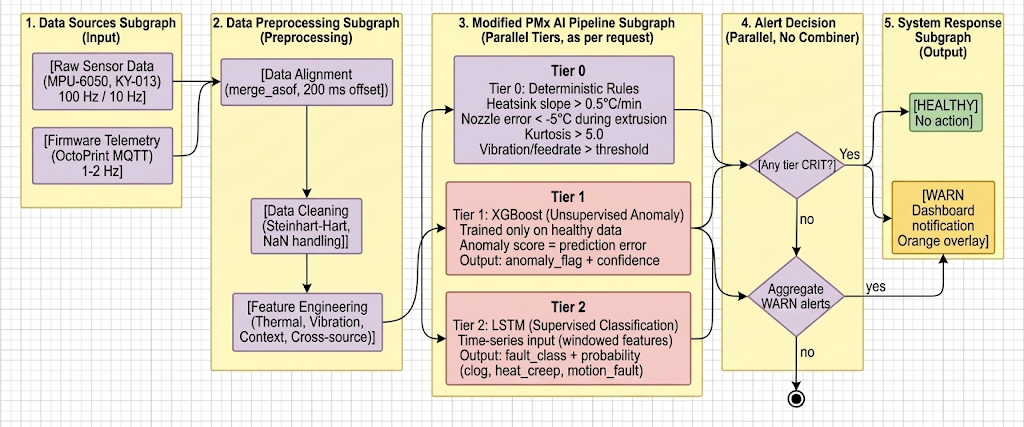
\includegraphics[width=0.9\textwidth]{figures/diagram_ia_pipeline}
    \caption{IA pipeline: from raw sensor data to alert generation}
    \label{fig:ia_pipeline}
\end{figure}

\textbf{Tier 0 (rules):} Uses deterministic thresholds. For heat creep: heatsink slope > 0.5°C per minute sustained. For clogging: nozzle error < -5°C during extrusion, or vibration kurtosis > 5.0.

\textbf{Tier 1 (Isolation Forest):} An unsupervised anomaly detection method \cite{liu2008isolation}. It is trained on healthy baseline data (at least 10 prints) and outputs an anomaly probability between 0 and 1.

\textbf{Tier 2 (XGBoost):} A supervised multi-class classifier that identifies specific faults (clog, heat creep, motion fault) \cite{chen2016xgboost}. It is trained on labelled events collected from Tier 0.

\textbf{Ensemble combiner:} Uses a weighted sum of active tiers. A final score below 0.3 means HEALTHY, between 0.3 and 0.7 means WARN, and 0.7 or above means CRIT (which triggers a print pause).

\subsection{Layer 4: Virtual Model Layer}

This layer combines a geometric model (the 3D visual representation) and a behavioural model (the health state). The geometric model is a glTF 2.0 file exported from Blender. The dynamic sub-model maintains instantaneous health, rolling statistics, and machine history (print sessions, faults, maintenance records).

\subsection{Layer 5: Supervision Layer}

A web-based dashboard built with Vite, React, and Three.js. It has three panels: a central 3D printer model, sensor charts on the left, and an alert feed on the right. CRIT alerts trigger an automatic print pause via the OctoPrint REST API.

\section{Geometric Modeling (The 3D Model)}

The 3D model of the BCN3D+ was created in Blender 4.x using reference photographs and technical drawings \cite{blender2024manual}. The model uses metric units (millimetres) so that OctoPrint coordinates map directly to object transformations. Components are named to match the FMEA classes: \texttt{extruder\_heatsink}, \texttt{nozzle\_assembly}, \texttt{x\_carriage}, \texttt{x\_belt}, \texttt{y\_belt}, and \texttt{z\_leadscrew}.

The model is exported as a glTF 2.0 binary file (.glb) \cite{khronos2022gltf} and served as a static asset. At runtime, Three.js updates the positions of moving parts.

\section{Behavioral Modeling (How the Twin Behaves)}

Behavioral modelling uses a hybrid grey-box approach that combines physics-based rules (which are interpretable and need no training) with data-driven machine learning (which learns complex patterns).

\subsection{Physics-Based Models}

\subsubsection{Thermal Model}
The nozzle is modelled as a first-order lumped system:
\[
\tau \frac{dT_n}{dt} = P_{heater}(t) - h_{tot}(T_n - T_{eq})
\]
Under normal PID control, the nozzle error stays within ±2°C. Heatsink temperature slope (how fast it heats up) is the primary indicator for heat creep. A sustained slope above 0.5°C per minute triggers a Tier 0 warning.

\subsubsection{Vibration Model}
The stepper motor excitation frequency is calculated from the feedrate and steps per millimetre. Belt resonance is approximated by a standard formula. Rather than predicting absolute values, the system monitors shifts in the dominant frequency.

\subsection{Data-Driven Models}

Isolation Forest requires no labels and runs efficiently on a Raspberry Pi. XGBoost handles supervised fault classification. The system also implements simple prognostics: for progressive faults like bearing wear or heat creep, a linear extrapolation of the trend over 30 minutes issues a predictive warning if the CRIT threshold is expected within 15 minutes.

\subsection{Adaptive Baseline}

At the start of each print, the system retrieves baseline RMS statistics from the last 10 healthy sessions and recalibrates thresholds dynamically. This adapts to machine aging and environmental changes.

\section{Real-Time Synchronisation}

Real-time synchronisation ensures the virtual model mirrors the physical printer at all times.

\subsection{Data Flow}
\begin{enumerate}
    \item The ESP8266 publishes sensor data at 2 Hz via MQTT.
    \item OctoPrint publishes telemetry at 1 to 5 Hz.
    \item The data aligner merges the streams (with a 200 ms shift and a tolerance window of ±500 ms).
    \item The PMx AI evaluates the tiers and generates alerts.
    \item A WebSocket bridge forwards the state to browser clients at 2 Hz.
    \item Three.js renders the visualisation at over 60 frames per second.
\end{enumerate}
End-to-end latency averages 280 to 500 milliseconds, well within the 10 second warning lead time needed for clogging detection.

\subsection{Bidirectional Connection}

Observation (from physical to virtual) is always active. Action (from virtual to physical) only occurs for CRIT alerts: the backend sends a pause command via the OctoPrint REST API. This qualifies the system as a true digital twin (bidirectional) in the Kritzinger taxonomy \cite{kritzinger2018digital}, not just a digital shadow.

\subsection{Synchronisation Metrics}
\begin{itemize}
    \item Latency: 280 to 500 milliseconds
    \item Virtual model update rate: 2 Hz
    \item MQTT QoS 0 loss rate: less than 1\%
    \item CRIT alert delivery: QoS 1 guaranteed
    \item Command response time (pause command): less than 500 milliseconds
\end{itemize}

\endinput